{{算法要求:}必须采用顺序存储结构。}

{{基本思路:}从表的一端开始,顺序扫描线性表,依次将扫描到的关键字和给定值k比较,若当前扫描的关键字与k相等,则查找成功;若扫描结束后,仍未有关键字与k相等,则查找失败。代码实现非常简单,如下:}{}

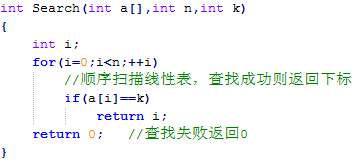
\includegraphics[width=3.70833in,height=1.69792in]{png-jpeg-pics/A6443AB171562CF2863483C88E45019D.png}
